\documentclass[12pt, letterpaper]{article}

% --- Packages ---
\usepackage{geometry}
 \geometry{margin=1in}
\usepackage{graphicx}
\usepackage{amsmath, amssymb}
\usepackage{booktabs}
\usepackage{hyperref}
\usepackage{cite}
\usepackage{setspace}
\onehalfspacing
\usepackage{fontspec}
\usepackage{polyglossia}
\usepackage{float}
\usepackage{svg}
\usepackage{enumitem}
\setmainlanguage{vietnamese}

\usepackage{listings}
\usepackage{xcolor}

\lstset{
    language=C,
    basicstyle=\ttfamily\small,
    keywordstyle=\color{blue},
    stringstyle=\color{red},
    commentstyle=\color{green!60!black},
    breaklines=true,
    frame=single, % Tạo khung xung quanh code
    backgroundcolor=\color{gray!5}
}

\renewcommand{\lstlistingname}{Mã nguồn}

% --- Metadata ---
\title{Giải bài tập 15}
\author{Đỗ Hoàng Gia Bảo - 23020783 \\ \small Khoa Điện tử - Viễn Thông}
\date{\today}

\begin{document}

\maketitle

\begin{abstract}
\begin{center}
    Báo cáo sẽ trình các bài tập số 1, 2 trang 43, 44  Bài-10
\end{center}
\end{abstract}
% --- Front Matter (Roman Numerals) ---
\newpage
\tableofcontents

% --- Main Content (Arabic Numerals) ---
\newpage
\pagenumbering{arabic}
\setcounter{page}{3} % This automatically resets the counter to 1

\section{Bài tập 1}
\subsection{Đề bài}
Ổ đĩa có 5000 trục rãnh đánh số từ 0 đến 4999. Đầu đọc/ghi 
đang ở trục rãnh 2150, nó vừa đáp ứng yêu cầu tại
trục rãnh 1085. Yêu cầu vào/ra các khối dữ liệu trên các
trục rãnh (theo trình tự FIFO) như sau: 2069, 1212,
2296, 2800, 544, 1618, 356, 1523, 4965, 3681.

Vẽ sơ đồ đường đi của đầu đọc/ghi và tính tổng quãng
đường di chuyển của đầu đọc/ghi cho các thuật toán lập
lịch sau:
\begin{enumerate}[label=\alph*.]
    \item SCAN
    \item C-SCAN
    \item LOOK
    \item C-LOOK
\end{enumerate}

\subsection{Giải bài tập}
\begin{enumerate}[label=\alph*.]
    \item SCAN
    
    Trong thuật toán SCAN, đầu đọc/ghi của ổ đĩa sẽ di chuyển từ một đầu 
    của ổ đĩa sang đầu kia, phục vụ tất cả các yêu cầu (requests) nằm 
    trên đường đi của nó. Khi đến đầu tận cùng của ổ đĩa 
    , đầu đọc sẽ đổi hướng và quay trở lại phía 
    ngược lại, tiếp tục phục vụ các yêu cầu còn lại.

    Vì đầu đọc/ghi đang ở trục rãnh 2150 và nó vừa đấp ứng yêu cầu trục 
    rãnh 1085, đầu đọc/ghi đang di chuyển về đầu rãnh 4999.

    Vì vậy sơ đồ đường đi của đầu đọc/ghi như sau:
    \begin{figure}[H]
        \centering
        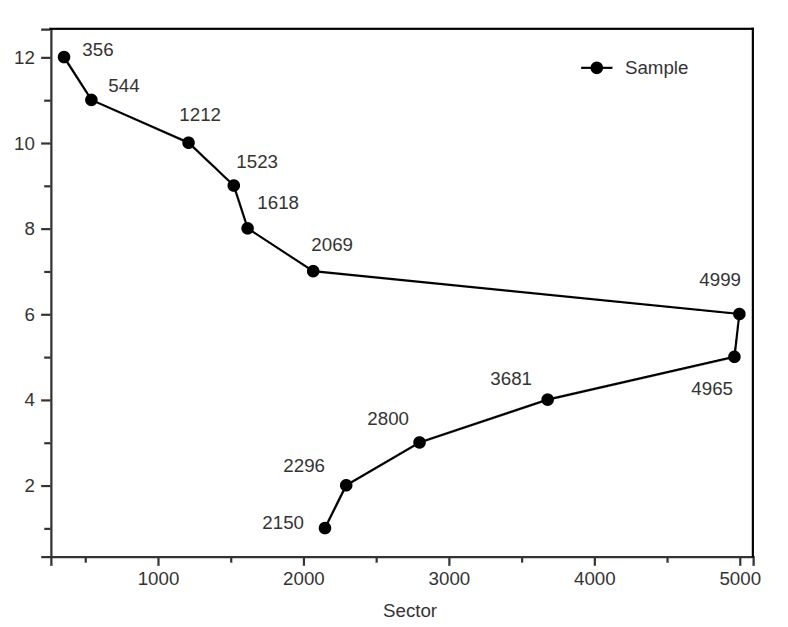
\includegraphics[width=1.0\textwidth]{Images/SCAN.jpg}
        \caption{Sơ đồ đường đi của thuật toán SCAN}
    \end{figure}
    
    Dựa vào sơ đồ trên, tổng quãng đường di chuyển của đầu đọc/ghi là:
    $$(4999 - 2150) + (4999 - 356) = 7492 \text{ rãnh}$$

    \item C-SCAN

    Trong thuật toán C-SCAN, đầu đọc sẽ di chuyển theo một chiều 
    (chiều tăng), phục vụ tất cả các yêu cầu trên đường đi cho đến tận 
    cùng của đĩa (trục rãnh 4999). Sau đó, nó lập tức quay ngoắt hành 
    trình về đầu tận cùng bên kia (trục rãnh 0) mà không phục vụ yêu 
    cầu nào trên đường quay về, rồi tiếp tục di chuyển theo chiều tăng 
    để phục vụ các yêu cầu còn lại.

    Vì vậy sơ đồ đường đi của đầu đọc/ghi như sau:
    \begin{figure}[H]
        \centering
        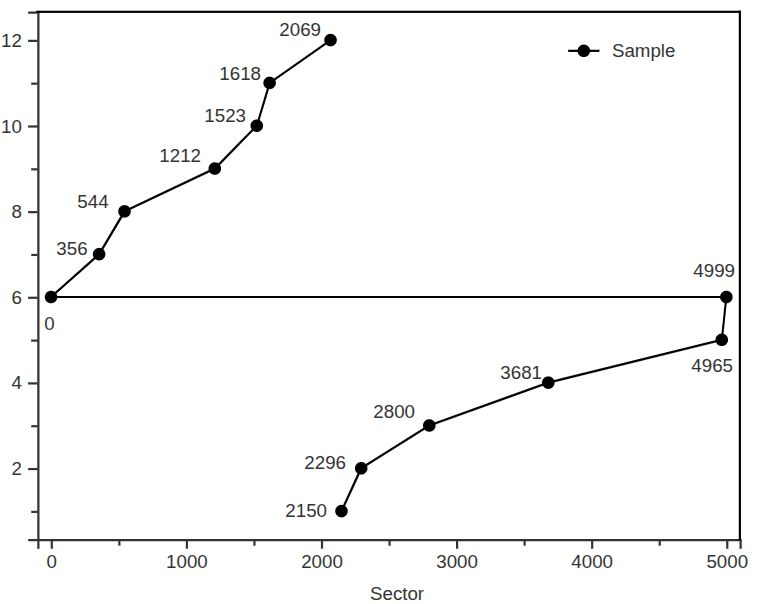
\includegraphics[width=1.0\textwidth]{Images/C_SCAN.jpg}
        \caption{Sơ đồ đường đi của thuật toán C-SCAN}
    \end{figure}

    Dựa vào sơ đồ trên, tổng quãng đường di chuyển của đầu đọc/ghi là:
    $$(4999 - 2150) + (2069 - 0) = 4918 \text{ rãnh}$$
    \item LOOK
    
    Thuật toán LOOK giống như SCAN nhưng thay vì đến các tận cùng của 
    ổ đĩa, nó chỉ đi đến trục rãnh có yêu cầu xa nhất chứ không chạy 
    cố đến tận cùng biên của đĩa (0 hoặc 4999) rồi mới quay đầu.

    Vì đầu đọc/ghi đang ở trục rãnh 2150 và nó vừa đấp ứng yêu cầu trục 
    rãnh 1085, đầu đọc/ghi đang di chuyển về đầu rãnh 4999.

    Vì vậy sơ đồ đường đi của đầu đọc/ghi như sau:
    \begin{figure}[H]
        \centering
        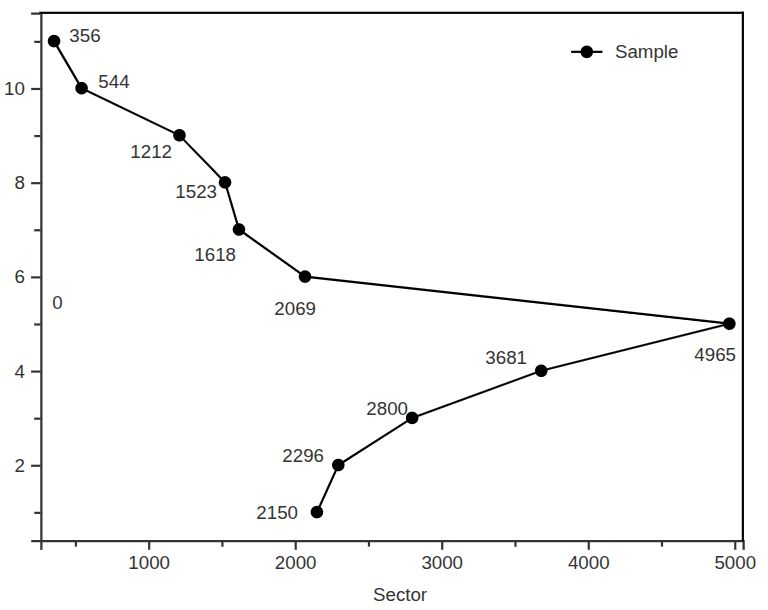
\includegraphics[width=1.0\textwidth]{Images/LOOK.jpg}
        \caption{Sơ đồ đường đi của thuật toán LOOK}
    \end{figure}

    Dựa vào sơ đồ trên, tổng quãng đường di chuyển của đầu đọc/ghi là:
    $$(4965 - 2150) + (4965 - 356) = 7424 \text{ rãnh}$$

    \item C-LOOK
    
    Thuật toán C-LOOK giống như C-SCAN nhưng nó chỉ đi đến trục 
    rãnh có yêu cầu lớn nhất xong quay lại yêu cầu nhỏ nhất.

    Vì vậy sơ đồ đường đi của đầu đọc/ghi như sau:
    \begin{figure}[H]
        \centering
        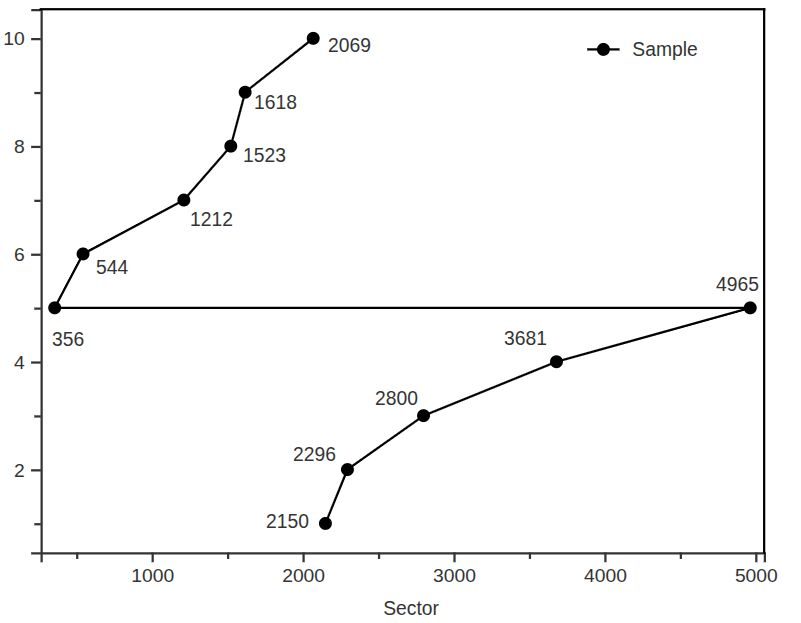
\includegraphics[width=1.0\textwidth]{Images/C_LOOK.jpg}
        \caption{Sơ đồ đường đi của thuật toán C-LOOK}
    \end{figure}

    Dựa vào sơ đồ trên, tổng quãng đường di chuyển của đầu đọc/ghi là:
    $$(4965 - 2150) + (2069 - 544) = 4340 \text{ rãnh}$$

\end{enumerate}
\section{Bài tập 2}
\subsection{Đề bài}
Một ổ cứng có các thông số sau:
\begin{itemize}
    \item Thời gian tìm kiếm track trung bình 10 ms, thời gian tìm kiếm
track liền kề 2 ms.
    \item Tốc độ trục quay (RPM): 800
    \item Số lượng sector mỗi track là 10
    \item Số byte mỗi sector là 4096
\end{itemize}
Tính tốc độ truyền dữ liệu.
\subsection{Giải bài tập}
Vì mỗi track có 10 sector và mỗi sector có thể lưu 4096 bytes, dung
lượng của mỗi track là:
$$\text{Dung lượng 1 track} = 10 \times 4096 = 40.960\text{ bytes}$$

Tiếp theo, vì đĩa quay với tốc độ 800 vòng trên phút nên tốc độ truyền
dữ liệu là:
$$ \text{Tốc độ truyền dữ liệu} = \text{Dung lượng của track} \times \text{tốc độ quay} $$
$$ \text{Tốc độ truyền dữ liệu} = 40960 \times \frac{800}{60} = 54613.3333333 \text{( bytes/s)} $$
\end{document}